\section{Empirical Monte Carlo Validation}\label{sec:simulation}

To test SACL and Synapticide's Law, we executed a 10,000-run Monte Carlo simulation sampling across heavy-tailed operational distributions.

\begin{figure}[htbp]
\centering
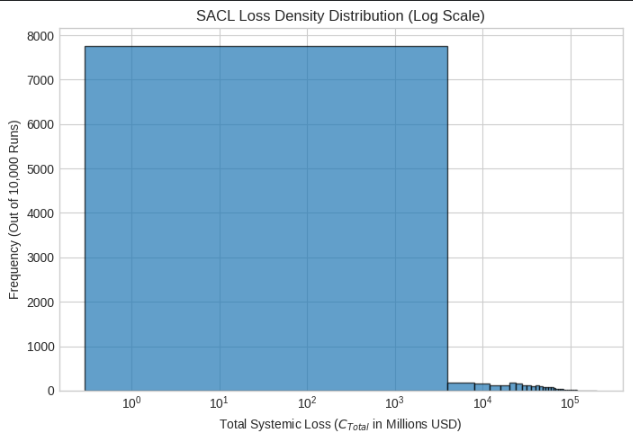
\includegraphics[width=0.48\textwidth]{figures/density_plot.png}
\caption{SACL Systemic Loss Density Distribution across 10,000 simulated breach runs, demonstrating Extreme Value Distribution (EVD) power-law behavior.}
\label{fig:density}
\end{figure}

\begin{figure}[htbp]
\centering
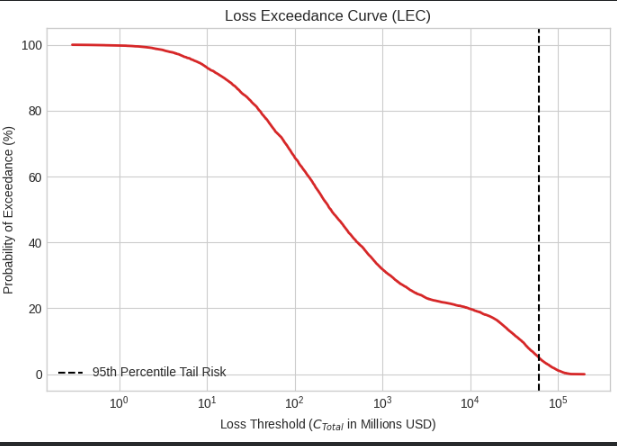
\includegraphics[width=0.48\textwidth]{figures/lec_curve.png}
\caption{Loss Exceedance Curve (LEC) illustrating probability of exceedance across financial loss thresholds, highlighting the 95th percentile tail risk at \$61.18B USD.}
\label{fig:lec}
\end{figure}

\subsection{Statistical Distribution Analysis}
As shown in Fig.~\ref{fig:density} and Fig.~\ref{fig:lec}, the empirical distribution confirms severe heavy-tailed characteristics:
\begin{itemize}
    \item \textbf{Median ($50^{\text{th}}$ Percentile):} \$258.24M USD
    \item \textbf{Upper Quartile ($75^{\text{th}}$ Percentile):} \$2.27B USD
    \item \textbf{Tail Risk ($95^{\text{th}}$ Percentile):} \$61.18B USD
    \item \textbf{Worst-Case ($99^{\text{th}}$ Percentile):} \$104.60B USD
\end{itemize}

The $\approx 236\times$ divergence between median breach expectations and the $95^{\text{th}}$ percentile tail risk empirically validates Axioms 1 and 2: when automated circuit breakers ($K_{\text{cb}}$) fail, velocity multipliers compound downstream supply chain disruption exponentially.